%* 
%* ------------------------------------------------------------------
%* FCF.tex - Freight Car Forwarder 2 user manual
%* Created by Robert Heller on Tue Aug  4 16:43:52 2009
%* ------------------------------------------------------------------
%* Modification History: $Log$
%* Modification History: Revision 1.1  2002/07/28 14:03:50  heller
%* Modification History: Add it copyright notice headers
%* Modification History:
%* ------------------------------------------------------------------
%* Contents:
%* ------------------------------------------------------------------
%*  
%*     Model RR System, Version 2
%*     Copyright (C) 1994,1995,2002-2005  Robert Heller D/B/A Deepwoods Software
%* 			51 Locke Hill Road
%* 			Wendell, MA 01379-9728
%* 
%*     This program is free software; you can redistribute it and/or modify
%*     it under the terms of the GNU General Public License as published by
%*     the Free Software Foundation; either version 2 of the License, or
%*     (at your option) any later version.
%* 
%*     This program is distributed in the hope that it will be useful,
%*     but WITHOUT ANY WARRANTY; without even the implied warranty of
%*     MERCHANTABILITY or FITNESS FOR A PARTICULAR PURPOSE.  See the
%*     GNU General Public License for more details.
%* 
%*     You should have received a copy of the GNU General Public License
%*     along with this program; if not, write to the Free Software
%*     Foundation, Inc., 675 Mass Ave, Cambridge, MA 02139, USA.
%* 
%*  
%* 

\documentclass[12pt,notitlepage,twoside]{book}
\usepackage{graphicx}
\usepackage{mathptm}
\usepackage{times}
\usepackage{makeidx}
\usepackage{url}
\usepackage{supertabular}
\usepackage{MyTitlepage}
\usepackage{listings}
\pagestyle{headings}
\makeindex
\emergencystretch=50pt
\begin{document}
\lstset{language=Tcl,basicstyle=\footnotesize,numbers=left,stepnumber=5}% Most examples will be in Tcl
\newcommand{\MRRSubTitle}{Freight Car Forwarder Manual}
%* 
%* ------------------------------------------------------------------
%* titlepage.tex - Common documentation title page
%* Created by Robert Heller on Sun Oct 13 15:59:49 2002
%* ------------------------------------------------------------------
%* Modification History: $Log$
%* Modification History: Revision 1.3  2007/10/22 17:17:27  heller
%* Modification History: 10222007
%* Modification History:
%* Modification History: Revision 1.2  2004/04/14 23:20:24  heller
%* Modification History: Updated copyright.
%* Modification History:
%* Modification History: Revision 1.1  2002/10/17 00:02:24  heller
%* Modification History: Documentation support files.
%* Modification History:
%* Modification History: Revision 1.1  2002/07/28 14:03:50  heller
%* Modification History: Add it copyright notice headers
%* Modification History:
%* ------------------------------------------------------------------
%* Contents:
%* ------------------------------------------------------------------
%*  
%*     Model RR System, Version 2
%*     Copyright (C) 1994,1995,2002  Robert Heller D/B/A Deepwoods Software
%* 			51 Locke Hill Road
%* 			Wendell, MA 01379-9728
%* 
%*     This program is free software; you can redistribute it and/or modify
%*     it under the terms of the GNU General Public License as published by
%*     the Free Software Foundation; either version 2 of the License, or
%*     (at your option) any later version.
%* 
%*     This program is distributed in the hope that it will be useful,
%*     but WITHOUT ANY WARRANTY; without even the implied warranty of
%*     MERCHANTABILITY or FITNESS FOR A PARTICULAR PURPOSE.  See the
%*     GNU General Public License for more details.
%* 
%*     You should have received a copy of the GNU General Public License
%*     along with this program; if not, write to the Free Software
%*     Foundation, Inc., 675 Mass Ave, Cambridge, MA 02139, USA.
%* 
%*  
%* 
%* 
%* $Id$  
%* 

\title{Model Railroad System \\ A collection of utilities for Model Railroaders\\ \MRRSubTitle}
\author{Robert Heller \\ Deepwoods Software \\ Wendell, MA, USA}
\date{\today}
\begin{titlepage}

\maketitle

%\begin{centering}
%\epsfig{file=../Cover1.ps} \\
%\end{centering}

\clearpage


This documentation was prepared with \LaTeX.

This document describes version 2 of the Model Railroad System package.

\vspace{.25in}



{\small Copyright \copyright 1994,1995,2002-2012 by Robert Heller D/B/A Deepwoods
Software}

\vspace{.25in}

All rights reserved.  Permission is granted to copy this document in
electronic form only, so long as it is with the software it
documents. 

The author, Robert Heller, may be contacted electronically (E-Mail) via
the following:

\begin{description}
\item[FidoNet] 1:321/153, Locks Hill BBS.
\item[InterNet] heller@deepsoft.com
\end{description}

Web site URL: {\tt http://www.deepsoft.com/}.

\thispagestyle{empty}
\setcounter{page}{0}
\clearpage

\end{titlepage}


\pagenumbering{roman}
\tableofcontents
\listoffigures
\listoftables
\cleardoublepage
%       
%%* 
%* ------------------------------------------------------------------
%* Preface.tex - Preface to the user manual
%* Created by Robert Heller on Sat Apr 21 10:32:44 2007
%* ------------------------------------------------------------------
%* Modification History: $Log$
%* Modification History: Revision 1.1  2007/05/06 12:49:40  heller
%* Modification History: Lock down  for 2.1.8 release candidate 1
%* Modification History:
%* Modification History: Revision 1.1  2002/07/28 14:03:50  heller
%* Modification History: Add it copyright notice headers
%* Modification History:
%* ------------------------------------------------------------------
%* Contents:
%* ------------------------------------------------------------------
%*  
%*     Model RR System, Version 2
%*     Copyright (C) 1994,1995,2002-2005  Robert Heller D/B/A Deepwoods Software
%* 			51 Locke Hill Road
%* 			Wendell, MA 01379-9728
%* 
%*     This program is free software; you can redistribute it and/or modify
%*     it under the terms of the GNU General Public License as published by
%*     the Free Software Foundation; either version 2 of the License, or
%*     (at your option) any later version.
%* 
%*     This program is distributed in the hope that it will be useful,
%*     but WITHOUT ANY WARRANTY; without even the implied warranty of
%*     MERCHANTABILITY or FITNESS FOR A PARTICULAR PURPOSE.  See the
%*     GNU General Public License for more details.
%* 
%*     You should have received a copy of the GNU General Public License
%*     along with this program; if not, write to the Free Software
%*     Foundation, Inc., 675 Mass Ave, Cambridge, MA 02139, USA.
%* 
%*  
%* 

\chapter*{Preface}
\markboth{PREFACE}{PREFACE}%
\addcontentsline{toc}{chapter}{Preface}
\label{chpt:Preface}
\typeout{$Id$}

This is the user manual for the Model Railroad system.  It is a ``work
in progress'' and I will be adding chapters as I write the various
self-contained ``main programs''.

%
\cleardoublepage
\pagenumbering{arabic}
%
%%* 
%* ------------------------------------------------------------------
%* Introduction.tex - Introduction
%* Created by Robert Heller on Thu Apr 19 14:24:42 2007
%* ------------------------------------------------------------------
%* Modification History: $Log$
%* Modification History: Revision 1.1  2007/05/06 12:49:38  heller
%* Modification History: Lock down  for 2.1.8 release candidate 1
%* Modification History:
%* Modification History: Revision 1.1  2002/07/28 14:03:50  heller
%* Modification History: Add it copyright notice headers
%* Modification History:
%* ------------------------------------------------------------------
%* Contents:
%* ------------------------------------------------------------------
%*  
%*     Model RR System, Version 2
%*     Copyright (C) 1994,1995,2002-2005  Robert Heller D/B/A Deepwoods Software
%* 			51 Locke Hill Road
%* 			Wendell, MA 01379-9728
%* 
%*     This program is free software; you can redistribute it and/or modify
%*     it under the terms of the GNU General Public License as published by
%*     the Free Software Foundation; either version 2 of the License, or
%*     (at your option) any later version.
%* 
%*     This program is distributed in the hope that it will be useful,
%*     but WITHOUT ANY WARRANTY; without even the implied warranty of
%*     MERCHANTABILITY or FITNESS FOR A PARTICULAR PURPOSE.  See the
%*     GNU General Public License for more details.
%* 
%*     You should have received a copy of the GNU General Public License
%*     along with this program; if not, write to the Free Software
%*     Foundation, Inc., 675 Mass Ave, Cambridge, MA 02139, USA.
%* 
%*  
%* 

\chapter{Introduction}
\label{chapt:Introduction}
\typeout{$Id$}

This manual presents some information about how to write programs that
use various parts of Model Railroad System to control and manage various
aspects of operating your model railroad.  The Model Railroad System
includes code that interfaces with special hardware, including the PI
Engineering Raildriver Console (see
Chapter~\ref{chapt:RaildriverServer}), a Bruce Chubb network of control
nodes (see  Chapter~\ref{chapt:CMRIProgramming}), and a Lenz XPressNet
network (see Chapter~\ref{chapt:XPressNetProgramming}).  Also included
are a collection of Tcl scripts that implement a collection of widgets
that are useful for various aspects of programming utilities for a model
railroad system.

%* 
%* ------------------------------------------------------------------
%* FCFTutorial.tex - Tutorial chapter for the Freight Car Forwarder (V2)
%* Created by Robert Heller on Sat Apr 21 11:17:20 2007
%* ------------------------------------------------------------------
%* Modification History: $Log$
%* Modification History: Revision 1.1  2007/05/06 12:49:40  heller
%* Modification History: Lock down  for 2.1.8 release candidate 1
%* Modification History:
%* Modification History: Revision 1.1  2002/07/28 14:03:50  heller
%* Modification History: Add it copyright notice headers
%* Modification History:
%* ------------------------------------------------------------------
%* Contents:
%* ------------------------------------------------------------------
%*  
%*     Model RR System, Version 2
%*     Copyright (C) 1994,1995,2002-2005  Robert Heller D/B/A Deepwoods Software
%* 			51 Locke Hill Road
%* 			Wendell, MA 01379-9728
%* 
%*     This program is free software; you can redistribute it and/or modify
%*     it under the terms of the GNU General Public License as published by
%*     the Free Software Foundation; either version 2 of the License, or
%*     (at your option) any later version.
%* 
%*     This program is distributed in the hope that it will be useful,
%*     but WITHOUT ANY WARRANTY; without even the implied warranty of
%*     MERCHANTABILITY or FITNESS FOR A PARTICULAR PURPOSE.  See the
%*     GNU General Public License for more details.
%* 
%*     You should have received a copy of the GNU General Public License
%*     along with this program; if not, write to the Free Software
%*     Foundation, Inc., 675 Mass Ave, Cambridge, MA 02139, USA.
%* 
%*  
%* 

\chapter{Freight Car Forwarder (V2) Tutorial}
\label{chpt:fcf:Tutorial}
\typeout{$Id$}


\index{Freight Car Forwarder!Tutorial|(} The Freight Car Forwarder is a
program designed to simulate freight car traffic on your model
railroad.  It does this by matching types of freight cars with
industries.  Specific types of freight cars are meant to carry specific
types of commodities and specific industries produce or consume
specific types of commodities.

The Freight Car Forwarder program uses a collection of data files,
which describe the system layout (system file), the industries
(industry file), the train that will move the cars (trains file), and
the cars themselves (the cars file).  There are some additional files,
including an owner's file and a car types file, as well as a file for
statistics.  All of these files are plain text files--See
Section~\ref{sect:fcf:Files} and  Section~\ref{sect:fcf:File Formats}
for more information on these files and their formats.

\section{Loading System Data}

The Freight Car Forwarder starts loading data by opening and reading
the system file, using either the file menu's \verb=Open...= item or open file
button on the toolbar.  This file contains the path names of the other
files, which are assumed to be relative to the directory (folder) that
contains the system file.  All of the system data is loaded into a
large data structure, which is then used by the program to simulate car
movements. Only car data is altered by the Freight Car Forwarder and the only
files that ever get re-written are the cars and statistics files.  The
other data files are never altered by the Freight Car Forwarder.  These
file can be edited using a plain text editor, such as Notepad
(MS-Windows) or Emacs (UNIX), should this be needed, as industries or
trains are added or removed, etc.

\section{Assigning Cars}

  In order to move cars, the cars need to be \emph{assigned}, that is, they
need to have a destination set, either to be loaded (if empty) or
unloaded (if loaded).  The Car Assignment procedure performs this task.

\section{Running Trains}

Once cars has been assigned, they need to be moved.  Cars are moved on
trains, and this is done with the run trains procedures.  There are
three of these procedures: Run All Trains in Operating Session, Run
Boxmoves, and Run One Train at a time.  The run trains procedures
simulate the actual movement of cars and determines which trains will
move which cars and in what order.  From this simulation, a set of yard
and switch lists can be generated and printed out for use during your
operating session.

\section{Printing Yard Lists}

Once the trains have been run, yard and switch lists can be printed
out, using the print yard lists menu.

\section{Generating Reports}

Various reports can also be generated and printed using the reports
menu. 

\section{Other activities}

Other activities include adding, removing, and editing cars and
displaying various state information, such as assigned and unassigned
cars, car movement information, lists of trains, and lists of
industries, stations, and divisions.
\index{Freight Car Forwarder!Tutorial|)} 

%* 
%* ------------------------------------------------------------------
%* FCFReference.tex - FCF V2 reference
%* Created by Robert Heller on Sat Apr 21 13:30:23 2007
%* ------------------------------------------------------------------
%* Modification History: $Log$
%* Modification History: Revision 1.1  2007/05/06 12:49:39  heller
%* Modification History: Lock down  for 2.1.8 release candidate 1
%* Modification History:
%* Modification History: Revision 1.1  2002/07/28 14:03:50  heller
%* Modification History: Add it copyright notice headers
%* Modification History:
%* ------------------------------------------------------------------
%* Contents:
%* ------------------------------------------------------------------
%*  
%*     Model RR System, Version 2
%*     Copyright (C) 1994,1995,2002-2005  Robert Heller D/B/A Deepwoods Software
%* 			51 Locke Hill Road
%* 			Wendell, MA 01379-9728
%* 
%*     This program is free software; you can redistribute it and/or modify
%*     it under the terms of the GNU General Public License as published by
%*     the Free Software Foundation; either version 2 of the License, or
%*     (at your option) any later version.
%* 
%*     This program is distributed in the hope that it will be useful,
%*     but WITHOUT ANY WARRANTY; without even the implied warranty of
%*     MERCHANTABILITY or FITNESS FOR A PARTICULAR PURPOSE.  See the
%*     GNU General Public License for more details.
%* 
%*     You should have received a copy of the GNU General Public License
%*     along with this program; if not, write to the Free Software
%*     Foundation, Inc., 675 Mass Ave, Cambridge, MA 02139, USA.
%* 
%*  
%* 

\chapter{Freight Car Forwarder (V2) Reference}
\label{chpt:fcf:Reference}
\typeout{$Id$}

The Freight Car Forwarder (V2) is a hybrid program, consisting of a
Tcl/Tk GUI on top of a C++ class library.  The GUI provides the user
interface to the algorithms and data structures contained in the C++
class library.

\section{Command Line Usage}

The name of the system file to load can be specified on the command
line. See Section~\ref{sect:fcf:loadsystem} for more information.

\section{Layout of the Main GUI}

\begin{figure}[hbpt]
\begin{centering}
\includegraphics[width=5in]{FCFMain.png}
\caption{The main GUI screen of the Freight Car Forwarder (V2) Program}
\label{fig:fcf:FCFMain}
\end{centering}
\end{figure}
\begin{figure}[hbpt]
\begin{centering}

\includegraphics[width=5in]{FCFMainToolbar.png}
\caption{The Toolbar of the Freight Car Forwarder (V2) Program}
\label{fig:fcf:FCFMainToolbar}
\end{centering}
\end{figure}
\begin{figure}[hbpt]
\begin{centering}
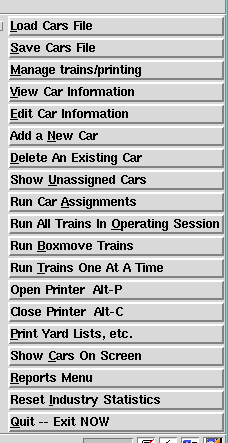
\includegraphics{FCFMainButtonMenu.png}
\caption{The Button Menu of the Freight Car Forwarder (V2) Program}
\label{fig:fcf:FCFMainButtonMenu}
\end{centering}
\end{figure}
\begin{figure}[hbpt]
\begin{centering}
\includegraphics{FCFMainIndicators.png}
\caption{The Indicators of the Freight Car Forwarder (V2) Program}
\label{fig:fcf:FCFMainIndicators}
\end{centering}
\end{figure}
The main GUI window\index{Freight Car Forwarder!main GUI}, show in
Figure~\ref{fig:fcf:FCFMain}, contains a menu bar, a toolbar
(Figure~\ref{fig:fcf:FCFMainToolbar}), a text display area, and a
button menu (Figure~\ref{fig:fcf:FCFMainButtonMenu}). There is also a 
work in progress message area, a  general status area, a progress
meter, and several indicators (Figure~\ref{fig:fcf:FCFMainIndicators}).
The main GUI also has three ``slide out'' frames, one for showing train
status when trains are run, one for viewing a car's information, and
one for editing a car's information. Each slide out has a corresponding
indicator. 

\section{Opening and loading a system file.}
\label{sect:fcf:loadsystem}
\index{Freight Car Forwarder!Loading a system file|(}

The \verb=File->Open...= menu button and the
\includegraphics{FCFLoadTool.png} toolbar button pop-up a file selection
dialog to select a system file to load. Once this file is successfully
loaded, the name of the file, the name of the system, the current
session and shift number, plus a count of  divisions, stations,
industries, cars, and trains is displayed in the main GUI's text area. 
Also all of the buttons are made active.  The name of the system file
can be specified on the command line and the named system file will be
loaded when the program starts.
\index{Freight Car Forwarder!Loading a system file|)}

\section{Loading and reloading the cars file.}

The \verb=Load Cars File= menu button and the

\includegraphics{FCFLoadCarsTool.png} toolbar button load (or reload)
the cars file.

\section{Saving the cars file.}

The \verb=Save Cars File= menu button and the 
\includegraphics{FCFSaveCarsTool.png} 
toolbar button save the cars and statistics files. This is something you
need to do after you have simulated a session, by running the car
assignment procedure and then run the trains in your session.  This
saves the state for the next time you run the Freight Car Forwarder.

\section{Managing trains and printing}
\begin{figure}[hbpt]
\begin{centering}
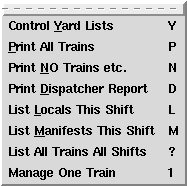
\includegraphics{FCFManageTrainsMenu.png}
\caption{Train/Printing Management Menu.}
\label{fig:fcf:FCFManageTrainsMenu}
\end{centering}
\end{figure}
The \verb=Manage trains/printing= menu button and the 

\includegraphics{FCFManageTrainsTool.png} toolbar button pop-up the
train/printing management menu.  This menu provides a set of functions
relating to what trains are printed and can also  print a dispatcher
report and generate lists of various sorts of trains.  The menu is shown
in  Figure~\ref{fig:fcf:FCFManageTrainsMenu}.

\subsection{Controling Yard Lists}

\begin{figure}[hbpt]
\begin{centering}
\includegraphics{FCFControlYardLDialog.png}
\caption{Control Yard Lists Dialog}
\label{fig:fcf:controlyardldialog}
\end{centering}
\end{figure}
The \verb=Control Yard Lists= menu item (y key) pops up a dialog, shown
in Figure~\ref{fig:fcf:controlyardldialog}, to control whether to print
0, 1, or 2 alphabetical lists and whether to print 0, 1, or 2 train
lists.

\subsection{Enabling printing for all trains}

The \verb=Print All Trains= menu item (p key) turns on printing for all
trains. 

\subsection{Disabling printing for all trains}

The \verb=Print No Trains= menu item (n key) turns off printing for all
trains.

\subsection{Printing a dispatcher report}

The \verb=Print Dispatcher Report= menu item (d key) enables the
printing of a dispatcher report.

\subsection{Listing local trains for this shift}

The \verb=List Locals This Shift= menu item (l key) lists all locals for
this shift.

\subsection{Listing manifests for this shift}

The \verb=List Manifests This Shift= menu item (m key) lists manifest
freights for this shift.

\subsection{Listing all trains for all shifts}

The \verb=List All Trains All Shifts= (? key) Lists all trains.

\subsection{Managing one train}

\begin{figure}[hbpt]
\begin{centering}
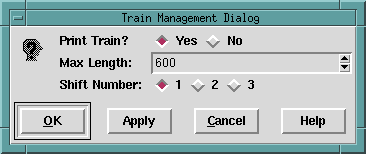
\includegraphics{FCFManage1TrainDialog.png}
\caption{Train Management Dialog}
\label{fig:fcf:manage1train}
\end{centering}
\end{figure}
The \verb=Manage One Train= menu item (1 key) pops up a dialog, shown
in Figure~\ref{fig:fcf:manage1train}, to enable or disable printing of
a single train, as well as setting the train's maximum length and
setting which shift the train will be run.  The train is selected with
the ``Select Train Dialog'', described in
Section~\ref{sect:fcf:selecttraindialog}.

\section{Viewing a car's information}

\begin{figure}[hbpt]
\begin{centering}
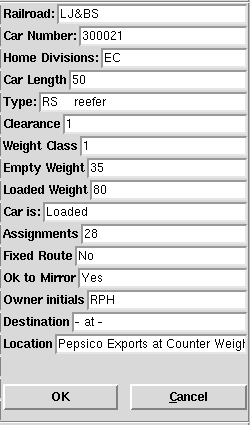
\includegraphics{FCFViewCarSlideout.png}
\caption{View Car Information Slideout}
\label{fig:fcf:viewcarslideout}
\end{centering}
\end{figure}
The \verb=View Car Information= menu button and the

\includegraphics{FCFViewCarTool.png} toolbar button display the
information about a single car.  The information is displayed on the
view car ``slide out'', shown in Figure~\ref{fig:fcf:viewcarslideout}.
The car is selected with the ``Search For Cars Dialog'', described in
Section~\ref{sect:fcf:searchcarsdialog}. 

\section{Editing a car's information}

\begin{figure}[hbpt]
\begin{centering}
\includegraphics{FCFEditCarSlideout.png}
\caption{Edit Car Information Slideout}
\label{fig:fcf:editcarslideout}
\end{centering}
\end{figure}
The \verb=Edit Car Information= menu button and the

\includegraphics{FCFEditCarTool.png} toolbar button display the
information about a single car and allow for editing this information. 
The information is displayed on the edit car ``slide out'', shown in
Figure~\ref{fig:fcf:editcarslideout}. The car is selected with the
``Search For Cars Dialog'', described in
Section~\ref{sect:fcf:searchcarsdialog}. 

\section{Adding a new car}

The \verb=Add a New Car= menu button and the

\includegraphics{FCFAddCarTool.png} toolbar button provide for adding a
new car.  The edit car ``slide out'', shown in
Figure~\ref{fig:fcf:editcarslideout} is displayed and the information
about the new car can be filled in and the car added.

\section{Deleting an existing car}

The \verb=Delete An Existing Car= menu button and the

\includegraphics{FCFDeleteCarTool.png} toolbar button provide for
deleting an existing car.  The car is selected with the ``Search For Cars
Dialog'', described in Section~\ref{sect:fcf:searchcarsdialog} and the
car's information is displayed in the view car ``slide out'', shown in
Figure~\ref{fig:fcf:viewcarslideout}. Actual removal can then be
confirmed.

\section{Showing cars without assignments}

The \verb=Show Unassigned Cars= menu button and the
\includegraphics{FCFShowUACarsTool.png} toolbar button display
unassigned cars in the text window.

\section{Running the car assignment procedure}

The \verb=Run Car Assignments= menu button and the

\includegraphics{FCFRunCarATool.png} toolbar button run the car
assignment procedure.  This procedure attempts to give as many
unassigned cars assignments, that is possible destinations. 
Considerations taken into account are the type of car, whether it is
loaded or not, industries with available trackage to accommodate the car,
and so on.  The list of cars is scanned twice and the progress of the
procedure is displayed in the text area.

\section{Running every train in the operating session}

\begin{figure}[hbpt]
\begin{centering}
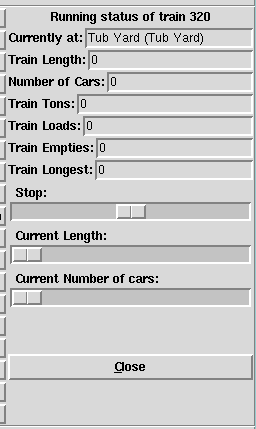
\includegraphics{FCFTrainStatusSlideout.png}
\caption{Train Status Slideout}
\label{fig:fcf:trainstatusslideout}
\end{centering}
\end{figure}
The \verb=Run All Trains in Operating Session= menu button and the
\includegraphics{FCFRunAllTrTool.png} toolbar button run all trains in
the operating session, except the end of session box moves.  Each
train's progress is shown in the ``Train Status Slideout'', shown in
Figure~\ref{fig:fcf:trainstatusslideout}.

\section{Running the boxmove trains}

The \verb=Run Boxmove Trains= menu button and the
\includegraphics{FCFRunBTrTool.png} toolbar button run all of the box
move trains in the operating session.  Each train's progress is shown
in the ``Train Status Slideout'', shown in
Figure~\ref{fig:fcf:trainstatusslideout}.

\section{Running a single train}

The \verb=Run Trains One At A Time= menu button and the

\includegraphics{FCFRun1TrTool.png} toolbar button run a single train,
selected with the ``Select Train Dialog'', described in
Section~\ref{sect:fcf:selecttraindialog}. The train's progress is shown
in the ``Train Status Slideout'', shown in
Figure~\ref{fig:fcf:trainstatusslideout}.


\section{Opening a Printer}

\begin{figure}[hbpt]
\begin{centering}
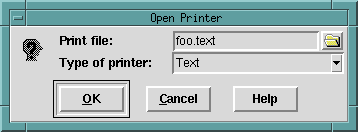
\includegraphics{FCFOpenPrinterDialog.png}
\caption{Open Printer Dialog}
\label{fig:fcf:openprinterdialog}
\end{centering}
\end{figure}
The \verb=Open Printer= menu button and the

\includegraphics{FCFOpenPrinterTool.png} toolbar button open the printer
output file, using the ``Open Printer Dialog'', shown in
Figure~\ref{fig:fcf:openprinterdialog}. The status of the printer
output, open or closed, is shown with the printer status indication,
\includegraphics{FCFPrinterInd.png}.

\section{Closing the printer}

The \verb=Close Printer= menu button and the

\includegraphics{FCFClosePrinterTool.png} toolbar button close the
printer.The status of the printer output, open or closed, is shown with
the printer status indication, \includegraphics{FCFPrinterInd.png}.

\section{Printing yard and switch lists}

The \verb=Print Yard Lists, etc.= menu button and the

\includegraphics{FCFPrintYardTool.png} toolbar button print the yard and
switch lists.

\section{Showing cars on the screen}

\begin{figure}[hbpt]
\begin{centering}
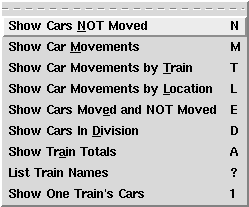
\includegraphics{FCFShowCarsMenu.png}
\caption{Show Cars Menu}
\label{fig:fcf:showcarsmenu}
\end{centering}
\end{figure}
The \verb=Show Cars On Screen= menu button and the
\includegraphics{FCFShowCarsTool.png} toolbar button pops up a menu,
shown in Figure~\ref{fig:fcf:showcarsmenu}, of classes of cars to show.

\section{Printing Reports}

\begin{figure}[hbpt]
\begin{centering}
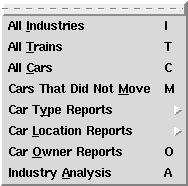
\includegraphics{FCFReportsMenu.png}
\caption{Reports Menu}
\label{fig:fcf:reportsmenu}
\end{centering}
\end{figure}
The \verb=Reports Menu= menu button and the
\includegraphics{FCFReportsTool.png} toolbar button pops up a menu,
shown in Figure~\ref{fig:fcf:reportsmenu}, of
possible reports.

\section{Reseting Industry Statistics}

The \verb=Reset Industry Statistics= menu button and the
\includegraphics{FCFResetStatsTool.png} toolbar button resets the
industry statistics.

\section{Quiting the application}

The \verb=Quit -- Exit NOW= menu button and the

\includegraphics{FCFCloseTool.png} toolbar button exit the program. A
confirmation dialog is popped up.


\section{General Dialogs}

\subsection{Control Yard Lists Dialog}
\subsection{Enter Owner Initials Dialog}

\subsection{Select A Train Dialog}
\label{sect:fcf:selecttraindialog}

\begin{figure}[hbpt]
\begin{centering}
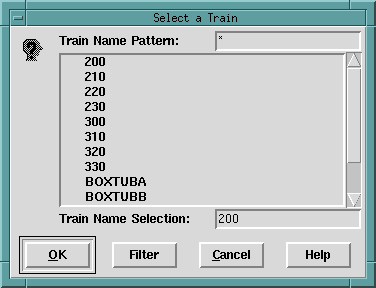
\includegraphics{FCFSelectATrainDialog.png}
\caption{Select A Train Dialog}
\label{fig:fcf:selecttraindialog}
\end{centering}
\end{figure}
The Select a Train Dialog is used to select a train (to manage, run, or
print). The \verb=Filter= button uses the Train Name Pattern to match
against train names to select a subset of trains to select from and can
contain these special sequences:  
\begin{itemize} 
\item \verb=*= Matches any sequence of zero or more characters in the
train name.
\item \verb=?= Matches any single character in the train name. 
\item \verb=[chars]= Matches any character in the set given by chars. 
If a sequence of the form \verb=x-y= appears in chars, then any
character between \verb=x= and  \verb=y=,  inclusive,  will match.
Characters are matched in a case insensitive way. 
\item \verb=\x= matches the single character \verb=x=. This provides a 
way of avoiding the special interpretation of the characters
\verb=*?[]\= in the pattern.
\end{itemize}

\subsection{Manage One Train Dialog}
\subsection{Open Printer Dialog}

\subsection{Search For Cars Dialog}
\label{sect:fcf:searchcarsdialog}

\begin{figure}[hbpt]
\begin{centering}
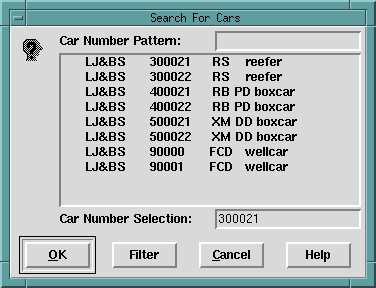
\includegraphics{FCFSelectACarDialog.png}
\caption{Search For Cars Dialog}
\label{fig:fcf:searchcarsdialog}
\end{centering}
\end{figure}
The Search For Cars Dialog is used to select a car (to view, edit, or
delete). The \verb=Filter= button selects a  subset of cars based on the
trailing car number digits.

\subsection{Select A Division Dialog}
\subsection{Select An Industry Dialog}
\subsection{Select A Station Dialog}
\subsection{Select Car Type}

\section{Data files}
\label{sect:fcf:Files}

The Freight Car Forwarder uses a collection of eight data files:

\begin{enumerate}
\item \verb=System File= This is the \textbf{master} file.  It contains the
(relative) paths to the remaining seven files, along with the name of
the railroad system, its divisions, and its stations.

\item \verb=Industry File= This file holds the description of the
industries, both on-line, which are actually modeled on the layout and
off- line, which are imaginary industries not actually on the layout,
but might be modeled as implied by staging yards or by interchange with
other layouts or imaginary off-line railroads.

\item \verb=Trains File= This file holds the description of the trains used
to actually move the cars about the layout.

\item \verb=Orders File= This file contains standing train orders and is
only used to add additional information to the printouts given to trail
operators.

\item \verb=Owners File= This file contains a mapping between owner initials
and owner names.  Used with various generated reports.

\item \verb=Car Types File= This file contains a mapping between car type
codes and full names and descriptions of car types.

\item \verb=Cars File= This is the file containing information about all of
the rolling stock on or off the layout.

\item \verb=Statistics File= This is the statistics file.  It is generated
by the program and contains statistical information about car and
industry utilization.
\end{enumerate}


\subsection{Data File Formats}
\label{sect:fcf:File Formats}

Some general notes:

A comment it indicated by an apostrophe.  All characters from the
apostrophe to the end of the line are discarded when read.  The files
generally contain lines of comma separated fields, a format
designed for BASIC read statements--the original program that this
program is based on was written in a version of BASIC and uses the same
file format.

\subsubsection{System File}

The first line of the system file is the name of the railroad system. 
This line is used in various banners and report headings.

The second line should be a blank line.

Then come the names of the remaining seven data files, one per line, in
this order: \verb=Industry File=, \verb=Trains File=, \verb=Orders File=, 
\verb=Owners File=, \verb=Car Types File=, \verb=Cars File=, and finally 
\verb=Statistics File=. 

After the file names comes the division list.  This starts with a count
of the maximum number of divisions:

\begin{verbatim}
Divisions = Number
\end{verbatim}

where Number is a positive non zero integer.

This is followed by division specifications, which is a list of 5 values
separated by commas:

\begin{verbatim}
Number,Symbol,Home,Area,Name
\end{verbatim}

Where Number is the index of the division (between 1 and the max number
of divisions, inclusive), Symbol is an alphanumeric character (a-z, 0-9,
A-Z), Home is the number of the home yard for this division (must be a
yard specified in the \verb=Industry File=), area is an Area symbol, and
Name is the name of the division.

A line containing a -1 terminates the list of divisions.

Then comes the stations (cities), starting with a line defining the maximum
number of stations:

\begin{verbatim}
Stations = Number
\end{verbatim}

where Number is a positive non zero integer.

This is followed by station specifications, which is a list of 4 values
separated by commas:

\begin{verbatim}
Number,Name,Division,Comment
\end{verbatim}

Where Number is the index of the station (between 1 and the max number
of stations, inclusive), Name is the name of the city, Division is the
division index, and Comment is commentary about the station. 
City/Station number one is used for the workbench.

A line containing a -1 terminates the list of stations.

\subsubsection{Industry File}

The industry file contains industries and yards.  The file starts with a
line specifying the maximum number of industries:

\begin{verbatim}
Industries = Number
\end{verbatim}

where Number is a positive non zero integer.

Followed by a line for each industry or yard.  Industry number 0 is
used for the repair yard, which is for cars not in service.  Each
industry's line contains these fields:

\begin{verbatim}
ID,T,STA,NAME,TLEN,ALEN,P,R,H,MIR,C,W,DCL,MAX,LD,EM
\end{verbatim}

Where:

\begin{description}
\item[ID]    Numeric identifier.
\item[T]     Types are \textbf{Y}ard or \textbf{I}ndustry or \textbf{O}ffline.
\item[STA]   Station Identifier.
\item[NAME]  User friendly place name.
\item[TLEN]  Actual or virtual track length.
\item[ALEN]  Assignable length.
\item[P]     Priority for car assignments. If \textbf{YARD} or \textbf{STAGE}, 
	\textbf{P} is $n$, the number of yard lists to print of type \verb=A=, 
	\verb=P=, or \verb=D=.
\item[R]     Reloads cars \textbf{Y}es or \textbf{N}o.
\item[H]     Hazard class for outbound cargo.
\item[MIR]   Mirror industry or 0 if none.
\item[C]     Maximum clearance plate.
\item[W]     Maximum weight class.
\item[DCL]   Destination Control List of divisions. If \textbf{YARD} or 
\textbf{STAGE}, DCL can contain:
  \begin{description}
  \item[A]     Alphabetical listing of cars in yard is permitted.
  \item[P]     Pickup listing of cars in yard is permitted.
  \item[D]     Dropoff listing of cars in yard is permitted.
  \end{description}
\item[MAX]   Maximum allowed car length.
\item[LD]    Loaded car types accepted.
\item[EM]    Empty car types accepted.
\end{description}

The industry listing is terminated by a line containing a -1.

\subsubsection{Trains File}

The trains file contains the trains used to move the cars.  The file
starts with a line specifying the maximum number of trains:

\begin{verbatim}
Trains = Number
\end{verbatim}

where Number is a positive non zero integer.

Followed by a record for each train (a newline is acceptable alternative
to a comma):

{\footnotesize
\begin{verbatim}
Number,Type,Shift,Done,Name,Maxcars, Divisions, Stops
	filler,Onduty,Print,Maxclear, Maxweight, Types,  Maxlen, 
	Description
\end{verbatim}
}

Where Number is the train number, Type is \textbf{M}anifest;
\textbf{B}oxmove; \textbf{W}ayfreight; or \textbf{P}assenger, Shift is
1; 2; or 3, Done is \textbf{Y}es or \textbf{N}o, Name is the train
name, Maxcars is the maximum number of cars, Divisions is a set of
division symbols or a wildcard (\verb=*=),Stops is a space separated
list of stations (Boxmove and Wayfrieghts) or industries (Manifests),
filler is an unused slot (use 0), Onduty is the time on duty (the
train's departure time) in the format HHMM, Print is \textbf{P}rint or
\textbf{N}oprint, Maxclear is the maximum clearance number, Maxweight
is the maximum weight number, Types is a set of car types this train
can carry, Maxlen is the maximum train length in feet, and Description
is a textual description of the train.

The train listing is terminated by a line containing a -1.

\subsubsection{Orders File}

This file contains lines with pairs:

\begin{verbatim}
Name,Order
\end{verbatim}

where Name is the name of a train and Order is a quoted string
containing the order.

\subsubsection{Owners File}

This file starts with a count of owners and then lines with with
triples:

\begin{verbatim}
Initials,Name,Comment
\end{verbatim}

where Initials are the three letter initials of an owner, Name is the
full name of the owner, and Comment is some descriptive text.

\subsubsection{Car Types File}

This is a file with exactly 91 records.  Each record contains:

\begin{verbatim}
Car Type Code,Car Type Group,Description,pad,Comment
\end{verbatim}

where Car Type Code is one of 91 printable characters, Car Type Group
is a single character, Description is a 16 character brief description,
pad is 0, and Comment is some descriptive text.

After the car types is the Car type groupings, which map groups of car
types into groups using the second single character, with lines
containing these fields:

\begin{verbatim}
Car Type Group,Description,Comment
\end{verbatim}

where Car Type Group is a single character, Description is a 16
character brief description, and Comment is some descriptive text.

\subsubsection{Cars File}

The cars file starts with three numbers, one per line:

\begin{verbatim}
Total shifts
Current shift
Max car count
\end{verbatim}

The first number is the total number of shifts, the second is the
current shift number (1, 2, or 3), and the third number is the maximum
number of cars in the file.

The remainder of the file is car records. This file must be kept in
[alphabetical order]! Each record contains:

{\footnotesize
\begin{verbatim}
Type,Marks,Number,Home,CarLen,ClearPlate,CarWeight,EmptyWt,
	LoadLimit,Loaded,Mirror?,Fixed?,Owner,Done,Last,Moves,Loc,
	Dest,NTrips,NAssigns
\end{verbatim}
}
Where Type is from car types file, Marks is the railroad reporting
marks (9 characters max), Number is the car number (8 characters max),
Home is car home division (from system file), CarLen is extreme car
length, ClearPlate is the clearance plate (from plate file), CarWeight
is car weight class (from weight file), EmptyWt is light weight in
tons, LoadLimit is load limit in tons, Loaded is \textbf{L}loaded or
\textbf{E}mpty, Mirror? is ok to mirror \textbf{Y}es or \textbf{N}o,
Fixed? is fixed route \textbf{Y}es or \textbf{N}o, Owner is car owner's
3 character initials (from owners file), Done is car is done moving for
this session \textbf{Y}es or \textbf{N}o, Last is last train to handle
the car from trains file,Moves is actual movements this session,Loc is
car's present location from industry file, Dest car's destination from
industry file, NTrips is number of car trips, and NAssigns is number of
car assignments.

\subsubsection{Statistics File}

The statistics is a file generated as an output and should not be hand
edited.  This file has two formats, V1 and V2.  V1 is the original
format used by the original BASIC program.  V2 is an improved version
that avoids getting the fields jammed together due to numerical overflow
(result numbers too large for the field sizes).

The first line of either format contains the statistics period number. 
If in the new format (V2), this number is followed by a comma.

The rest of file file contains lines of four numbers, either space
separated (V1) or comma separated (V2): industry index, car count, car
length, and statistics length.

\subsubsection{Other data files}

There are some additional data files, which are not actually loaded into
the system.  These are the plate, weight, and hazard files.  These are
just informational files that are used to map clearance plate, weight
class, and hazard levels of cars.



\chapter{Help}

This help window contains some basic navigation features.  There are
buttons for traversing the history stack.  There are also key bindings
within the help window itself:

\begin{description}
\item[s] Search forward.  Searches forward in the text for the next
occurance of the specificed text.
\item[r] Search backward.  Searches backward in the text for the next
occurance of the specificed text.
\item[f] History forward.  Goes to the next page in the history stack.
\item[b] History backward. Goes to the previous page in the history
stack.
\item[Tab] Next link. Goes to the next hyperlink.
\item[Control-Tab] Previous link. Goes to the previous hyperlink.
\end{description}




\chapter*{Copying}
\addcontentsline{toc}{chapter}{Copying}
\markboth{Copying}{Copying}
\begin{verbatim}
		    GNU GENERAL PUBLIC LICENSE
		       Version 2, June 1991

 Copyright (C) 1989, 1991 Free Software Foundation, Inc.
     59 Temple Place, Suite 330, Boston, MA  02111-1307  USA
 Everyone is permitted to copy and distribute verbatim copies
 of this license document, but changing it is not allowed.

			    Preamble

  The licenses for most software are designed to take away your
freedom to share and change it.  By contrast, the GNU General Public
License is intended to guarantee your freedom to share and change free
software--to make sure the software is free for all its users.  This
General Public License applies to most of the Free Software
Foundation's software and to any other program whose authors commit to
using it.  (Some other Free Software Foundation software is covered by
the GNU Library General Public License instead.)  You can apply it to
your programs, too.

  When we speak of free software, we are referring to freedom, not
price.  Our General Public Licenses are designed to make sure that you
have the freedom to distribute copies of free software (and charge for
this service if you wish), that you receive source code or can get it
if you want it, that you can change the software or use pieces of it
in new free programs; and that you know you can do these things.

  To protect your rights, we need to make restrictions that forbid
anyone to deny you these rights or to ask you to surrender the rights.
These restrictions translate to certain responsibilities for you if you
distribute copies of the software, or if you modify it.

  For example, if you distribute copies of such a program, whether
gratis or for a fee, you must give the recipients all the rights that
you have.  You must make sure that they, too, receive or can get the
source code.  And you must show them these terms so they know their
rights.

  We protect your rights with two steps: (1) copyright the software, and
(2) offer you this license which gives you legal permission to copy,
distribute and/or modify the software.

  Also, for each author's protection and ours, we want to make certain
that everyone understands that there is no warranty for this free
software.  If the software is modified by someone else and passed on, we
want its recipients to know that what they have is not the original, so
that any problems introduced by others will not reflect on the original
authors' reputations.

  Finally, any free program is threatened constantly by software
patents.  We wish to avoid the danger that redistributors of a free
program will individually obtain patent licenses, in effect making the
program proprietary.  To prevent this, we have made it clear that any
patent must be licensed for everyone's free use or not licensed at all.

  The precise terms and conditions for copying, distribution and
modification follow.
\end{verbatim}
\clearpage
\begin{verbatim}
		    GNU GENERAL PUBLIC LICENSE
   TERMS AND CONDITIONS FOR COPYING, DISTRIBUTION AND MODIFICATION

  0. This License applies to any program or other work which contains
a notice placed by the copyright holder saying it may be distributed
under the terms of this General Public License.  The "Program", below,
refers to any such program or work, and a "work based on the Program"
means either the Program or any derivative work under copyright law:
that is to say, a work containing the Program or a portion of it,
either verbatim or with modifications and/or translated into another
language.  (Hereinafter, translation is included without limitation in
the term "modification".)  Each licensee is addressed as "you".

Activities other than copying, distribution and modification are not
covered by this License; they are outside its scope.  The act of
running the Program is not restricted, and the output from the Program
is covered only if its contents constitute a work based on the
Program (independent of having been made by running the Program).
Whether that is true depends on what the Program does.

  1. You may copy and distribute verbatim copies of the Program's
source code as you receive it, in any medium, provided that you
conspicuously and appropriately publish on each copy an appropriate
copyright notice and disclaimer of warranty; keep intact all the
notices that refer to this License and to the absence of any warranty;
and give any other recipients of the Program a copy of this License
along with the Program.

You may charge a fee for the physical act of transferring a copy, and
you may at your option offer warranty protection in exchange for a fee.

  2. You may modify your copy or copies of the Program or any portion
of it, thus forming a work based on the Program, and copy and
distribute such modifications or work under the terms of Section 1
above, provided that you also meet all of these conditions:

    a) You must cause the modified files to carry prominent notices
    stating that you changed the files and the date of any change.

    b) You must cause any work that you distribute or publish, that in
    whole or in part contains or is derived from the Program or any
    part thereof, to be licensed as a whole at no charge to all third
    parties under the terms of this License.

    c) If the modified program normally reads commands interactively
    when run, you must cause it, when started running for such
    interactive use in the most ordinary way, to print or display an
    announcement including an appropriate copyright notice and a
    notice that there is no warranty (or else, saying that you provide
    a warranty) and that users may redistribute the program under
    these conditions, and telling the user how to view a copy of this
    License.  (Exception: if the Program itself is interactive but
    does not normally print such an announcement, your work based on
    the Program is not required to print an announcement.)
\end{verbatim}
\clearpage
\begin{verbatim}
These requirements apply to the modified work as a whole.  If
identifiable sections of that work are not derived from the Program,
and can be reasonably considered independent and separate works in
themselves, then this License, and its terms, do not apply to those
sections when you distribute them as separate works.  But when you
distribute the same sections as part of a whole which is a work based
on the Program, the distribution of the whole must be on the terms of
this License, whose permissions for other licensees extend to the
entire whole, and thus to each and every part regardless of who wrote it.

Thus, it is not the intent of this section to claim rights or contest
your rights to work written entirely by you; rather, the intent is to
exercise the right to control the distribution of derivative or
collective works based on the Program.

In addition, mere aggregation of another work not based on the Program
with the Program (or with a work based on the Program) on a volume of
a storage or distribution medium does not bring the other work under
the scope of this License.

  3. You may copy and distribute the Program (or a work based on it,
under Section 2) in object code or executable form under the terms of
Sections 1 and 2 above provided that you also do one of the following:

    a) Accompany it with the complete corresponding machine-readable
    source code, which must be distributed under the terms of Sections
    1 and 2 above on a medium customarily used for software interchange; or,

    b) Accompany it with a written offer, valid for at least three
    years, to give any third party, for a charge no more than your
    cost of physically performing source distribution, a complete
    machine-readable copy of the corresponding source code, to be
    distributed under the terms of Sections 1 and 2 above on a medium
    customarily used for software interchange; or,

    c) Accompany it with the information you received as to the offer
    to distribute corresponding source code.  (This alternative is
    allowed only for noncommercial distribution and only if you
    received the program in object code or executable form with such
    an offer, in accord with Subsection b above.)

The source code for a work means the preferred form of the work for
making modifications to it.  For an executable work, complete source
code means all the source code for all modules it contains, plus any
associated interface definition files, plus the scripts used to
control compilation and installation of the executable.  However, as a
special exception, the source code distributed need not include
anything that is normally distributed (in either source or binary
form) with the major components (compiler, kernel, and so on) of the
operating system on which the executable runs, unless that component
itself accompanies the executable.

If distribution of executable or object code is made by offering
access to copy from a designated place, then offering equivalent
access to copy the source code from the same place counts as
distribution of the source code, even though third parties are not
compelled to copy the source along with the object code.
\end{verbatim}
\clearpage
\begin{verbatim}
  4. You may not copy, modify, sublicense, or distribute the Program
except as expressly provided under this License.  Any attempt
otherwise to copy, modify, sublicense or distribute the Program is
void, and will automatically terminate your rights under this License.
However, parties who have received copies, or rights, from you under
this License will not have their licenses terminated so long as such
parties remain in full compliance.

  5. You are not required to accept this License, since you have not
signed it.  However, nothing else grants you permission to modify or
distribute the Program or its derivative works.  These actions are
prohibited by law if you do not accept this License.  Therefore, by
modifying or distributing the Program (or any work based on the
Program), you indicate your acceptance of this License to do so, and
all its terms and conditions for copying, distributing or modifying
the Program or works based on it.

  6. Each time you redistribute the Program (or any work based on the
Program), the recipient automatically receives a license from the
original licensor to copy, distribute or modify the Program subject to
these terms and conditions.  You may not impose any further
restrictions on the recipients' exercise of the rights granted herein.
You are not responsible for enforcing compliance by third parties to
this License.

  7. If, as a consequence of a court judgment or allegation of patent
infringement or for any other reason (not limited to patent issues),
conditions are imposed on you (whether by court order, agreement or
otherwise) that contradict the conditions of this License, they do not
excuse you from the conditions of this License.  If you cannot
distribute so as to satisfy simultaneously your obligations under this
License and any other pertinent obligations, then as a consequence you
may not distribute the Program at all.  For example, if a patent
license would not permit royalty-free redistribution of the Program by
all those who receive copies directly or indirectly through you, then
the only way you could satisfy both it and this License would be to
refrain entirely from distribution of the Program.

If any portion of this section is held invalid or unenforceable under
any particular circumstance, the balance of the section is intended to
apply and the section as a whole is intended to apply in other
circumstances.

It is not the purpose of this section to induce you to infringe any
patents or other property right claims or to contest validity of any
such claims; this section has the sole purpose of protecting the
integrity of the free software distribution system, which is
implemented by public license practices.  Many people have made
generous contributions to the wide range of software distributed
through that system in reliance on consistent application of that
system; it is up to the author/donor to decide if he or she is willing
to distribute software through any other system and a licensee cannot
impose that choice.

This section is intended to make thoroughly clear what is believed to
be a consequence of the rest of this License.
\end{verbatim}
\clearpage
\begin{verbatim}
  8. If the distribution and/or use of the Program is restricted in
certain countries either by patents or by copyrighted interfaces, the
original copyright holder who places the Program under this License
may add an explicit geographical distribution limitation excluding
those countries, so that distribution is permitted only in or among
countries not thus excluded.  In such case, this License incorporates
the limitation as if written in the body of this License.

  9. The Free Software Foundation may publish revised and/or new versions
of the General Public License from time to time.  Such new versions will
be similar in spirit to the present version, but may differ in detail to
address new problems or concerns.

Each version is given a distinguishing version number.  If the Program
specifies a version number of this License which applies to it and "any
later version", you have the option of following the terms and conditions
either of that version or of any later version published by the Free
Software Foundation.  If the Program does not specify a version number of
this License, you may choose any version ever published by the Free Software
Foundation.

  10. If you wish to incorporate parts of the Program into other free
programs whose distribution conditions are different, write to the author
to ask for permission.  For software which is copyrighted by the Free
Software Foundation, write to the Free Software Foundation; we sometimes
make exceptions for this.  Our decision will be guided by the two goals
of preserving the free status of all derivatives of our free software and
of promoting the sharing and reuse of software generally.
\end{verbatim}
\addcontentsline{toc}{section}{Warranty}
\begin{verbatim}
			    NO WARRANTY

  11. BECAUSE THE PROGRAM IS LICENSED FREE OF CHARGE, THERE IS NO WARRANTY
FOR THE PROGRAM, TO THE EXTENT PERMITTED BY APPLICABLE LAW.  EXCEPT WHEN
OTHERWISE STATED IN WRITING THE COPYRIGHT HOLDERS AND/OR OTHER PARTIES
PROVIDE THE PROGRAM "AS IS" WITHOUT WARRANTY OF ANY KIND, EITHER EXPRESSED
OR IMPLIED, INCLUDING, BUT NOT LIMITED TO, THE IMPLIED WARRANTIES OF
MERCHANTABILITY AND FITNESS FOR A PARTICULAR PURPOSE.  THE ENTIRE RISK AS
TO THE QUALITY AND PERFORMANCE OF THE PROGRAM IS WITH YOU.  SHOULD THE
PROGRAM PROVE DEFECTIVE, YOU ASSUME THE COST OF ALL NECESSARY SERVICING,
REPAIR OR CORRECTION.

  12. IN NO EVENT UNLESS REQUIRED BY APPLICABLE LAW OR AGREED TO IN WRITING
WILL ANY COPYRIGHT HOLDER, OR ANY OTHER PARTY WHO MAY MODIFY AND/OR
REDISTRIBUTE THE PROGRAM AS PERMITTED ABOVE, BE LIABLE TO YOU FOR DAMAGES,
INCLUDING ANY GENERAL, SPECIAL, INCIDENTAL OR CONSEQUENTIAL DAMAGES ARISING
OUT OF THE USE OR INABILITY TO USE THE PROGRAM (INCLUDING BUT NOT LIMITED
TO LOSS OF DATA OR DATA BEING RENDERED INACCURATE OR LOSSES SUSTAINED BY
YOU OR THIRD PARTIES OR A FAILURE OF THE PROGRAM TO OPERATE WITH ANY OTHER
PROGRAMS), EVEN IF SUCH HOLDER OR OTHER PARTY HAS BEEN ADVISED OF THE
POSSIBILITY OF SUCH DAMAGES.

		     END OF TERMS AND CONDITIONS
\end{verbatim}
\clearpage
\begin{verbatim}
	    How to Apply These Terms to Your New Programs

  If you develop a new program, and you want it to be of the greatest
possible use to the public, the best way to achieve this is to make it
free software which everyone can redistribute and change under these terms.

  To do so, attach the following notices to the program.  It is safest
to attach them to the start of each source file to most effectively
convey the exclusion of warranty; and each file should have at least
the "copyright" line and a pointer to where the full notice is found.

    <one line to give the program's name and a brief idea of what it does.>
    Copyright (C) <year>  <name of author>

    This program is free software; you can redistribute it and/or modify
    it under the terms of the GNU General Public License as published by
    the Free Software Foundation; either version 2 of the License, or
    (at your option) any later version.

    This program is distributed in the hope that it will be useful,
    but WITHOUT ANY WARRANTY; without even the implied warranty of
    MERCHANTABILITY or FITNESS FOR A PARTICULAR PURPOSE.  See the
    GNU General Public License for more details.

    You should have received a copy of the GNU General Public License
    along with this program; if not, write to the Free Software
    Foundation, Inc., 59 Temple Place, Suite 330, Boston, MA  02111-1307  USA


Also add information on how to contact you by electronic and paper mail.

If the program is interactive, make it output a short notice like this
when it starts in an interactive mode:

    Gnomovision version 69, Copyright (C) year  name of author
    Gnomovision comes with ABSOLUTELY NO WARRANTY; for details type `show w'.
    This is free software, and you are welcome to redistribute it
    under certain conditions; type `show c' for details.

The hypothetical commands `show w' and `show c' should show the appropriate
parts of the General Public License.  Of course, the commands you use may
be called something other than `show w' and `show c'; they could even be
mouse-clicks or menu items--whatever suits your program.

You should also get your employer (if you work as a programmer) or your
school, if any, to sign a "copyright disclaimer" for the program, if
necessary.  Here is a sample; alter the names:

  Yoyodyne, Inc., hereby disclaims all copyright interest in the program
  `Gnomovision' (which makes passes at compilers) written by James Hacker.

  <signature of Ty Coon>, 1 April 1989
  Ty Coon, President of Vice

This General Public License does not permit incorporating your program into
proprietary programs.  If your program is a subroutine library, you may
consider it more useful to permit linking proprietary applications with the
library.  If this is what you want to do, use the GNU Library General
Public License instead of this License.
\end{verbatim}

\include{FCF_Version}
\cleardoublepage
\bibliography{MRR}
\bibliographystyle{plain}
\cleardoublepage
\printindex
\end{document}



